\subsubsection{Return paths between digits in the same row}
The gadgets of this class hold a increment/copy signal and the regional index
of the next digit to read. The height of these gadgets is dependent on $l$.
These gadgets are used so that upon writing a digit, the counter is able to
move back down to the next digit in the current row, and continue reading.
\vspace{1cm}

\begin{figure}[H]
    \centering
    \begin{subfigure}[t]{0.32\textwidth}
        \centering
        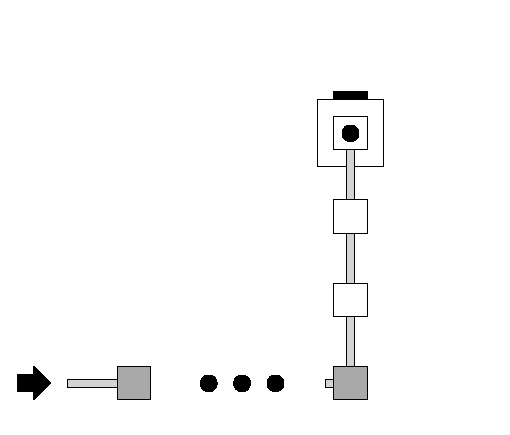
\includegraphics[width=0.24\textwidth]{cross_to_next_row}
        \caption{\label{fig:cross_to_next_row} {\tt Cross\_To\_Next\_Row}}
    \end{subfigure}%
    ~
    \begin{subfigure}[t]{0.32\textwidth}
        \centering
        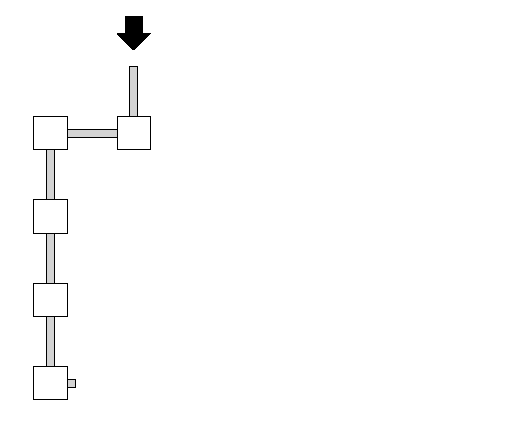
\includegraphics[width=0.24\textwidth]{exit_row_from_digit_1_or_digit_2}
        \caption{\label{fig:exit_row_from_digit_1_or_digit_2} {\tt Exit\_Row\_From\_Digit\_1\_Or\_2} }
    \end{subfigure}%
    ~
    \begin{subfigure}[t]{0.32\textwidth}
        \centering
        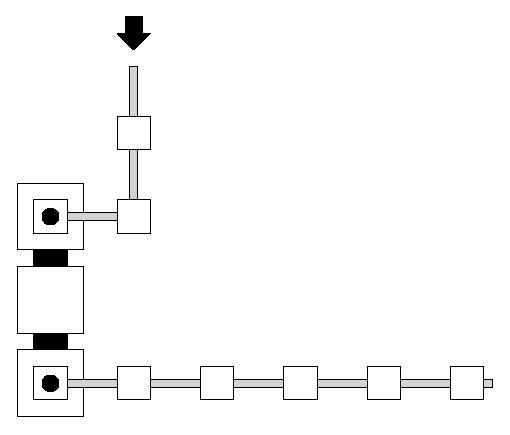
\includegraphics[width=0.24\textwidth]{exit_row_from_digit_3}
        \caption{\label{fig:exit_row_from_digit_3} {\tt Exit\_Row\_From\_Digit\_3}}
    \end{subfigure}%
    ~
\end{figure}


\begin{figure}[H]
    \centering
    \begin{subfigure}[t]{0.2\textwidth}
        \centering
        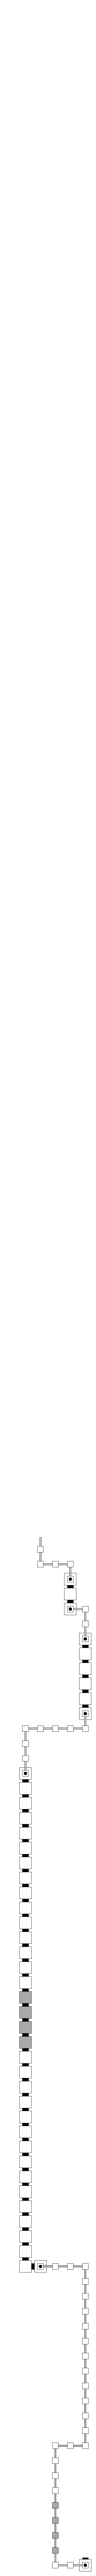
\includegraphics[width=0.2\textwidth]{return_paths/return_digit1_read_digit2_general}
        \caption{\label{fig:return_digit1_read_digit2_general} Return digit 1 read digit 2}
    \end{subfigure}%
    ~
    \begin{subfigure}[t]{0.2\textwidth}
        \centering
        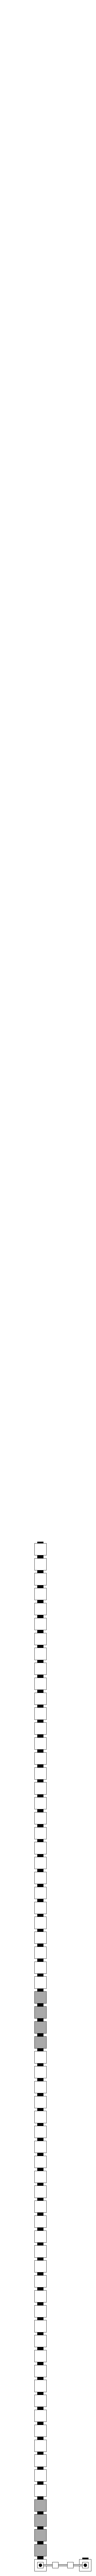
\includegraphics[width=0.2\textwidth]{return_paths/return_digit1_read_digit2_case2_msr}
        \caption{\label{fig:return_digit1_read_digit2_case2_msr} Return digit 1 read digit 2 -- Case 2}
    \end{subfigure}%
    ~
    \begin{subfigure}[t]{0.2\textwidth}
        \centering
        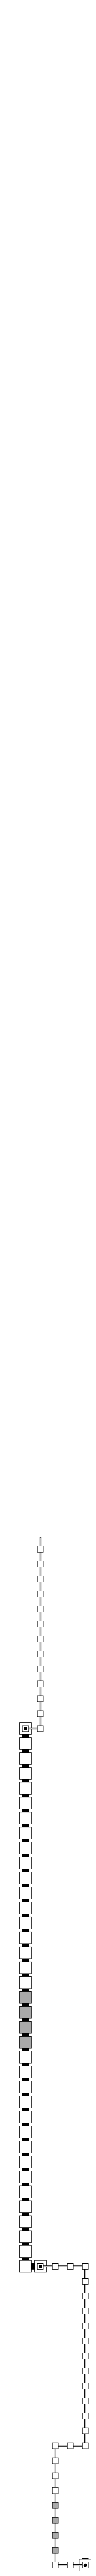
\includegraphics[width=0.2\textwidth]{return_paths/return_digit2_read_digit3_general}
        \caption{\label{fig:return_digit2_read_digit3_general} Return digit 2 read digit 3}
    \end{subfigure}%
    ~
    \begin{subfigure}[t]{0.2\textwidth}
        \centering
        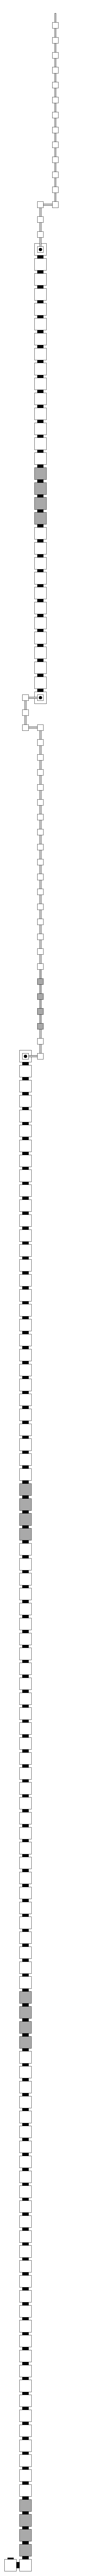
\includegraphics[width=0.2\textwidth]{return_paths/return_digit3_read_digit1_general}
        \caption{\label{fig:return_digit3_read_digit1_general} Return digit 3 read digit 1}
    \end{subfigure}%
    \caption{\label{fig:return_path_same_row} {\tt Return\_From\_Digit\_Read\_Digit} gadgets. These gadgets assemble north to south, starting on the south side of a digit top.}
\end{figure}

\noindent For each {\inc} $\in \{ {\tt increment, copy } \}$.

% todo yes/no?: pass L as input since gadget size is O(L), but inputs/outputs don't depend on it

\begin{itemize}
    \item Create
    $\begin{aligned}[t]
        \returnfromdonereaddtwo(& \left \langle {\tt ReturnD1ReadD2},          \inc \right\rangle,
                                  \left \langle {\tt DigitReader}, 2, \lambda, \inc \right\rangle \;)
    \end{aligned}$ \\ from the general gadget in Figure~\ref{fig:return_digit1_read_digit2_general}

    \item Create
    $\begin{aligned}[t]
        \returnfromdonereaddtwocasetwo(& \left\langle {\tt ReturnD1ReadD2-Case2},    \inc \right\rangle, \\
                                       & \left\langle {\tt DigitReader}, 2, \lambda, \inc \right\rangle \;)
    \end{aligned}$ \\ from the general gadget in Figure~\ref{fig:return_digit1_read_digit2_case2_msr}

    \item Create
    $\begin{aligned}[t]
        \returnfromdtworeaddthree(& \left\langle {\tt ReturnD2ReadD3},           \inc \right\rangle,
                                    \left\langle {\tt DigitReader},  3, \lambda, \inc \right\rangle \;)
    \end{aligned}$ \\ from the general gadget in Figure~\ref{fig:return_digit2_read_digit3_general}

    \item Create
    $\begin{aligned}[t]
            \returnfromdthreereaddone(& \left \langle {\tt ReturnD3ReadD1},           \inc \right\rangle,
                                        \left \langle {\tt DigitReader},  1, \lambda, \inc \right\rangle \;)
    \end{aligned}$ \\ from the general gadget in Figure~\ref{fig:return_digit3_read_digit1_general}

\end{itemize}


